% ============================================================
% Evaluación 01 — Cableado UTP Cat5e
% Reporte de práctica: ponchado y armado de un cable de par trenzado
% Redes de Comunicaciones de Datos (6.º semestre)
% UAZ · Unidad Académica de Ingeniería Eléctrica
% Ing. Electrónica Industrial con especialidad en Telecomunicaciones
% ============================================================
\documentclass[11pt,a4paper]{article}

\usepackage[utf8]{inputenc}
\usepackage[T1]{fontenc}
\usepackage[spanish,mexico]{babel}
\usepackage{graphicx}
\usepackage[margin=2.5cm]{geometry}
\usepackage{setspace}
\usepackage{parskip}
\usepackage{fancyhdr}
\usepackage{amsmath}
\usepackage{booktabs}
\usepackage{tabularx}
\usepackage[hidelinks]{hyperref}
\usepackage{xurl}

\onehalfspacing
\setlength{\parskip}{6pt}

\setlength{\headheight}{40pt}
\pagestyle{fancy}
\fancyhf{}
\fancyhead[L]{
\includegraphics[width=1cm]{../../../Assets/UIE.png}}
\fancyfoot[C]{\thepage}
\renewcommand{\headrulewidth}{0.4pt}

\begin{document}

% ---------------------------- PORTADA -----------------------
\begin{titlepage}
  \thispagestyle{empty}
  \begin{center}
    \vspace*{1cm}
    
\includegraphics[width=4.5cm]{../../../Assets/uaz.png}
    \vspace{0.8cm}

    {\large Universidad Autónoma de Zacatecas}\\[4pt]
    {\large Unidad Académica de Ingeniería Eléctrica}\\[4pt]
    {\normalsize Ingeniería Electrónica Industrial con especialidad en Telecomunicaciones}

    \vspace{1.8cm}
    {\LARGE\bfseries Evaluación 01}\\[10pt]
    {\Large\bfseries Cableado UTP Cat5e:\\[4pt] fundamento físico, ponchado y verificación}
  \end{center}

  \vspace{2.2cm}
  \begin{center}
    \begin{tabular}{rl}
      \textbf{Materia:} & Redes de Comunicaciones de Datos\\
      \textbf{Docente:} & José Ricardo Gómez Rodríguez\\
      \textbf{Alumno:}  & Arnold Yovick Ríos Zaldívar\\
      \textbf{Fecha:}   & Septiembre de 2026\\
    \end{tabular}
  \end{center}
  \vfill
\end{titlepage}

% ------------------------- INTRODUCCIÓN ---------------------
\section{Introducción}

Toda red de área local (LAN) descansa, en su nivel más elemental, sobre un
medio físico que transporta señales eléctricas entre dispositivos. Aunque lo
inalámbrico y la fibra óptica ganan terreno, el cable de par trenzado sin
blindaje (\textit{Unshielded Twisted Pair}, UTP) sigue siendo el medio
dominante en el cableado horizontal de oficinas, laboratorios y escuelas, por
su bajo costo, su facilidad de instalación y la madurez de sus estándares.

El presente reporte documenta el armado y ponchado de un cable UTP categoría
5e (\textit{Cat5e}) con conectores RJ-45 bajo la norma \textbf{T568B}. Más
allá de la destreza manual, la práctica tiene un fundamento electromagnético:
la geometría retorcida de los conductores no es un capricho de fabricación,
sino un mecanismo deliberado de cancelación de ruido. Por ello el reporte
explica primero \emph{por qué} el cable es de par trenzado, qué afectaciones
mitiga y cuáles son sus límites de distancia y velocidad; después describe el
procedimiento de ponchado y presenta la evidencia; y cierra vinculando la
teoría con los hallazgos prácticos y con las razones que justifican el uso de
Cat5e en entornos de red concretos.

% -------------------------- OBJETIVOS -----------------------
\section{Objetivos}

\subsection*{Objetivo general}

Armar y poner a prueba un cable UTP Cat5e con conectores RJ-45 bajo la norma
T568B, comprender el fundamento físico del trenzado y verificar el
cumplimiento de las especificaciones de distancia y velocidad de su categoría.

\subsection*{Objetivos específicos}

\begin{itemize}
  \item Explicar el principio de cancelación de ruido del par trenzado y las
        interferencias que mitiga (diafonía, EMI y RFI).
  \item Identificar la distancia máxima de canal (100~m) y las velocidades
        soportadas por la categoría 5e (hasta 1~Gbps) con base en los
        estándares vigentes.
  \item Ejecutar correctamente el orden de colores T568B y el proceso de
        crimpado de un latiguillo de red.
  \item Relacionar la teoría del cableado estructurado con la práctica y
        justificar la elección de Cat5e en entornos específicos.
\end{itemize}

% ------------------------ MARCO TEÓRICO ---------------------
\section{Marco teórico}

\subsection{¿Por qué es un par trenzado?}

Un cable UTP está formado por cuatro pares de conductores de cobre;
cada par transporta la señal de forma \textbf{diferencial}: la misma
información viaja en un hilo como tensión positiva y en su compañero como
tensión negativa, con corrientes iguales y de sentido opuesto. Esta simetría
es la clave del diseño. Cuando un campo electromagnético externo —proveniente
de un motor, un balasto fluorescente o un cable de potencia cercano— incide
sobre el par, induce prácticamente la \emph{misma} tensión de ruido en ambos
hilos, porque están físicamente juntos. A este componente idéntico se le llama
\textbf{ruido en modo común}. En el receptor se alimenta a un amplificador
diferencial, que resta las dos tensiones: la señal útil, de signo opuesto, se
suma; el ruido, idéntico en ambos, se cancela, de modo que
$V_{\text{recibida}} = (V_{+} + V_{n}) - (V_{-} + V_{n}) = V_{+} - V_{-}$.

Además del efecto diferencial, el trenzado aporta una segunda cancelación de
tipo geométrico. Al retorcerse los hilos, el área de la espira que forman se
invierte cada media vuelta; el voltaje inducido por un campo externo en una
espira tiene signo opuesto al inducido en la siguiente, de modo que los
voltajes inducidos a lo largo del par se cancelan entre sí. Por último, cada
par del cable se trenza con un \textbf{paso de trenzado distinto} (número de
vueltas por unidad de longitud), lo que evita que los pares queden paralelos
—condición que favorecería el acoplamiento mutuo— y reduce la diafonía
interna. En resumen, el trenzado convierte el cable en una estructura
intrínsecamente inmune al ruido, sin necesidad de blindaje metálico.

\subsection{Tipos de afectaciones que mitiga}

El diseño de par trenzado y el balanceo de los conductores combaten
principalmente las siguientes interferencias:

\begin{itemize}
  \item \textbf{Diafonía o \textit{crosstalk}}: es el acoplamiento inductivo y
        capacitivo entre pares vecinos del mismo cable. Se manifiesta como
        \textit{NEXT} (\textit{Near-End Crosstalk}, en el extremo cercano al
        transmisor), \textit{FEXT} (\textit{Far-End Crosstalk}, en el extremo
        lejano), \textit{ACR} (relación atenuación/diafonía),
        \textit{PS-NEXT} (\textit{Power Sum}, la suma de la interferencia de
        todos los pares) y \textit{diafonía ajena} o \textit{alien crosstalk},
        proveniente de cables adyacentes dentro de una canaleta.
  \item \textbf{Interferencia electromagnética (EMI)}: la radiación de
        equipos eléctricos y electrónicos —motores, variadores, fuentes
        conmutadas, líneas de potencia— que induce corrientes parásitas sobre
        los conductores.
  \item \textbf{Interferencia de radiofrecuencia (RFI)}: señales de radio,
        telefonía móvil y otros transmisores que el cable puede captar como
        una antena accidental.
  \item \textbf{Ruido en modo común y diferencias de potencial de tierra}:
        tensiones indeseadas que aparecen por igual en ambos conductores y
        que el receptor diferencial rechaza de forma natural.
\end{itemize}

El balanceo de los pares es tan importante que los estándares no solo fijan
los límites de NEXT y EMI, sino también la uniformidad del paso de trenzado:
cuanto mayor es el balanceo, menos energía irradia el cable hacia afuera
(\textit{emisión}) y menos capta desde afuera (\textit{susceptibilidad}).

\subsection{Distancia máxima: 100 metros}

Los estándares de cableado estructurado ANSI/TIA-568.2-D e ISO/IEC~11801
definen una \textbf{distancia máxima de canal de 100~m} para el cobre de par
trenzado, cifra compuesta por el enlace permanente horizontal (máximo 90~m,
del \textit{patch panel} del cuarto de telecomunicaciones a la toma de
usuario) más hasta 10~m de latiguillos (\textit{patch cords}), 5~m por
extremo. El límite responde a un compromiso entre atenuación y diafonía: al
crecer la longitud, la señal se debilita y la diafonía se hace relativamente
mayor, de modo que la \textit{relación señal a ruido} cae por debajo de lo que
exige la norma. Superar los 100~m impide garantizar el funcionamiento y
certificar el enlace.

\subsection{Velocidades de transmisión y categorías}

La categoría del cable determina su \textit{ancho de banda} (frecuencia
máxima certificada, en MHz) y, con ello, las velocidades que puede soportar.
La Tabla~\ref{tab:cat} resume las categorías de par trenzado más empleadas y
su desempeño según los estándares vigentes.

\begin{table}[htbp]
  \centering
  \small
  \begin{tabularx}{\textwidth}{l c c X}
    \toprule
    \textbf{Categoría} & \textbf{Ancho de banda} & \textbf{Velocidad típica} & \textbf{Estándar de Ethernet asociado} \\
    \midrule
    Cat3  & 16~MHz  & 10~Mbps                     & 10BASE-T \\
    Cat5  & 100~MHz & 100~Mbps                    & 100BASE-TX \\
    \textbf{Cat5e} & \textbf{100~MHz} & \textbf{1~Gbps (100~m)} & \textbf{1000BASE-T (IEEE 802.3ab)} \\
    Cat6  & 250~MHz & 1~Gbps (100~m); 10~Gbps (55~m) & 1000BASE-T / 10GBASE-T \\
    Cat6A & 500~MHz & 10~Gbps (100~m)             & 10GBASE-T \\
    \bottomrule
  \end{tabularx}
  \caption{Categorías de par trenzado, ancho de banda y velocidades de
  transmisión asociadas. La categoría 5e es la empleada en esta práctica.}
  \label{tab:cat}
\end{table}

La categoría 5e (\textit{enhanced}) conserva el mismo ancho de banda nominal
de 100~MHz que la Cat5, pero sus especificaciones eléctricas son más
estrictas: límites más severos de NEXT, PS-NEXT, pérdida de retorno y
atenuación, y un balanceo mejorado. Estas exigencias adicionales son las que
permiten garantizar la transmisión de \textbf{1~Gbps} mediante el estándar
IEEE~802.3ab (1000BASE-T) a la distancia completa de 100~m. A diferencia de
100BASE-TX, que emplea solo dos pares en un sentido, 1000BASE-T utiliza los
cuatro pares simultáneamente en modo bidireccional, con codificación
multi-nivel (PAM-5) y técnicas de cancelación de eco; de ahí que requiera
cables con bajos niveles de diafonía, precisamente la mejora que introduce la
categoría 5e.

\subsection{Norma de ponchado T568B}

El orden en que se acomodan los ocho hilos dentro del conector RJ-45 está
normalizado. La norma \textbf{T568B}, la más difundida en América, se resume
en la Tabla~\ref{tab:t568b}. Los pares funcionales conmutan de posición
respecto de la T568A: en la T568B el par naranja ocupa los pines 1--2 y el par
verde los pines 3--6, mientras que en la T568A ocurre lo contrario. Un cable
recto (\textit{patch}) usa la misma norma en ambos extremos; un cable cruzado
usa una norma distinta en cada extremo, práctica casi en desuso porque los
dispositivos modernos implementan autodetección (\textit{Auto-MDI/MDIX}).

\begin{table}[htbp]
  \centering
  \small
  \begin{tabular}{c l l}
    \toprule
    \textbf{Pin} & \textbf{Color (T568B)} & \textbf{Función de par} \\
    \midrule
    1 & Blanco--Naranja & Par 2 (TX+) \\
    2 & Naranja        & Par 2 (TX$-$) \\
    3 & Blanco--Verde  & Par 3 (RX+) \\
    4 & Azul           & Par 1 (BI)  \\
    5 & Blanco--Azul   & Par 1 (BI)  \\
    6 & Verde          & Par 3 (RX$-$) \\
    7 & Blanco--Café   & Par 4 (BI)  \\
    8 & Café           & Par 4 (BI)  \\
    \bottomrule
  \end{tabular}
  \caption{Asignación de pines y colores bajo la norma T568B, empleada en la
  práctica (BI = bidireccional en 1000BASE-T).}
  \label{tab:t568b}
\end{table}

% ------------------------- METODOLOGÍA ----------------------
\section{Metodología y desarrollo de la práctica}

\subsection{Materiales y herramientas}

Cable UTP categoría 5e (cuatro pares de cobre), dos conectores RJ-45 macho,
crimpadora de RJ-45, pelacables, tijeras de corte y probador de continuidad
(\textit{tester}) de red.

\subsection{Procedimiento de ponchado}

El armado se realizó de forma secuencial y simétrica en ambos extremos del
cable, siguiendo la norma T568B:

\begin{enumerate}
  \item \textbf{Pelado de la cubierta}: se retiró aproximadamente 2--3~cm de
        la funda exterior cuidando no dañar el aislamiento de los conductores.
  \item \textbf{Separación y destrenzado}: se separaron los cuatro pares y se
        destrenzaron únicamente el tramo necesario, para no alterar el paso de
        trenzado más de lo imprescindible.
  \item \textbf{Ordenamiento de colores}: se ordenaron los ocho hilos según la
        secuencia T568B —Blanco--Naranja, Naranja, Blanco--Verde, Azul,
        Blanco--Azul, Verde, Blanco--Café, Café— (Tabla~\ref{tab:t568b}).
  \item \textbf{Recorte e inserción}: se emparejaron y recortaron los hilos a
        ras y se deslizaron dentro del conector RJ-45 hasta que cada conductor
        alcanzara el fondo, verificando la secuencia a través del cuerpo
        transparente del conector.
  \item \textbf{Crimpado}: se ejerció presión firme con la crimpadora para
        que los contactos dorados perforaran el aislamiento de cada hilo y se
        fijara el retén sobre la cubierta.
  \item \textbf{Verificación}: se repitió el procedimiento en el extremo
        opuesto y se comprobó la continuidad de los ocho conductores con el
        probador, verificando que los ocho indicadores luminosos respondieran
        en el orden correcto (1 a 8).
\end{enumerate}

\subsection{Resultados}

La práctica concluyó con la elaboración de latiguillos de red funcionales,
verificados eléctricamente con el probador de continuidad. La
Figura~\ref{fig:grupal} presenta la evidencia fotográfica grupal de la
práctica, en la que se observa al equipo sosteniendo los cables armados.

\begin{figure}[htbp]
  \centering
  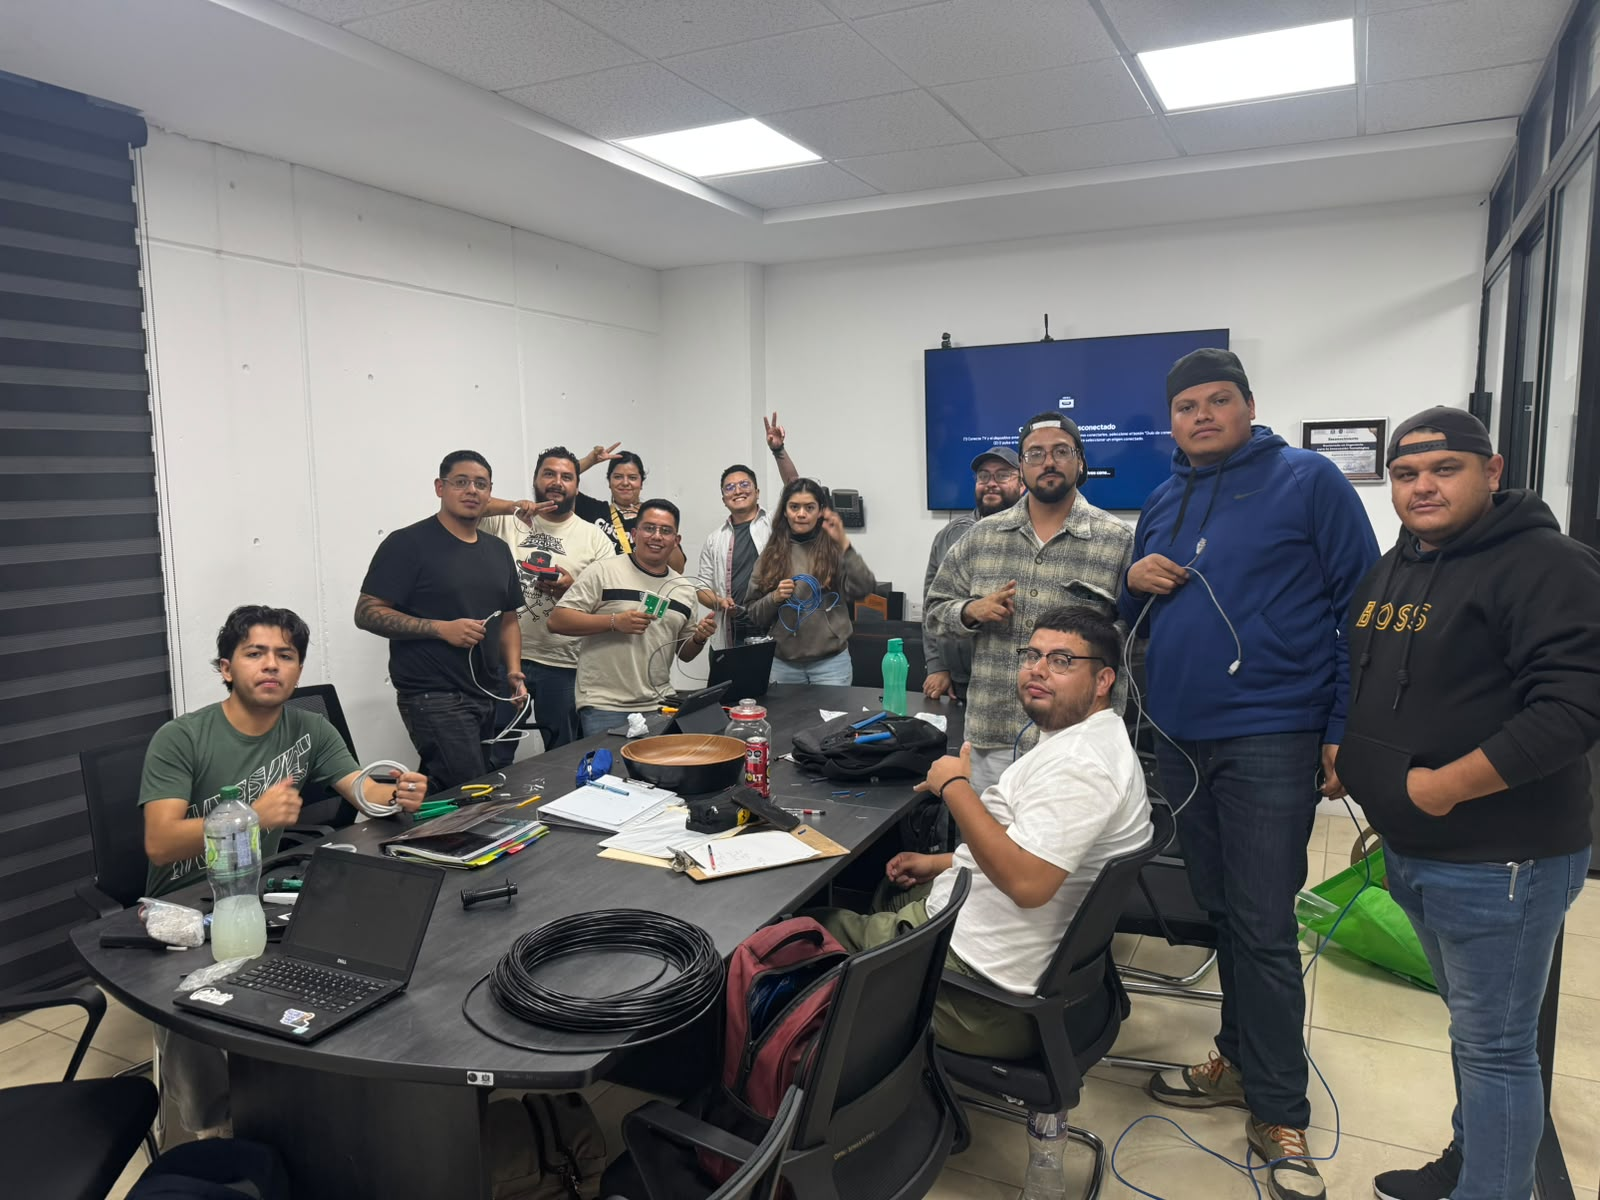
\includegraphics[width=0.78\textwidth]{img/grupal.jpeg}
  \caption{Evidencia fotográfica de la práctica de cableado UTP Cat5e: el
  equipo sostiene los latiguillos armados y ponchados bajo la norma T568B.}
  \label{fig:grupal}
\end{figure}

% ------------------------- DISCUSIÓN ------------------------
\section{Discusión: teoría y práctica}

La experiencia práctica confirma los conceptos del marco teórico. Al
destrenzar los conductores solo el tramo imprescindible para insertarlos en el
conector se respetó la razón física del diseño: cada destrenzado innecesario
aumenta el área expuesta al acoplamiento electromagnético y degrada la
cancelación de ruido, elevando la diafonía \cite{tia}. Del mismo modo, el paso
de trenzado distinto de cada par explica por qué no deben intercambiarse hilos
entre pines de forma caprichosa: hacerlo rompe la simetría diferencial que
permite rechazar el ruido en modo común.

La elección de la categoría 5e responde a un análisis costo--beneficio
adecuado a los entornos de red típicos de esta materia y del laboratorio. Un
canal de Cat5e certificado soporta \textbf{Gigabit Ethernet (1000BASE-T)} a
100~m, lo que cubre con holgura las necesidades de un aula, una oficina o un
laboratorio de cómputo donde el tráfico predominante es acceso a Internet,
transferencia de archivos y servicios locales. Para distancias horizontales
que rara vez superan los 90~m y velocidades que no rebasan 1~Gbps, la Cat5e
resulta suficiente y considerablemente más económica que la Cat6A necesaria
para 10~Gbps a 100~m. Su uso se justifica, además, porque es compatible
\textit{hacia atrás} con categorías inferiores y admite alimentación por
Ethernet (\textit{PoE}, IEEE~802.3af/at) para teléfonos IP, cámaras y puntos
de acceso inalámbrico, un requisito habitual en instalaciones modernas.

Los hallazgos prácticos también ilustran los límites del medio: el probador
solo confirma continuidad y orden de pines, pero no certifica parámetros
eléctricos como NEXT o pérdida de retorno, para lo cual se requiere un
certificador de enlaces. Por eso un cable que «suena bien» con un tester
básico puede no alcanzar 1~Gbps en un tramo largo: la continuidad es
condición necesaria, pero no suficiente, para cumplir la norma.

% -------------------------- CONCLUSIÓN ----------------------
\section{Conclusión}

Se armó y verificó correctamente un cable UTP Cat5e con conectores RJ-45 bajo
la norma T568B, cumpliendo los objetivos planteados. La práctica permitió
comprender que el par trenzado es una solución de ingeniería al problema del
ruido: la simetría diferencial de los conductores y la inversión del área de
espira en cada vuelta cancelan tanto el ruido en modo común —EMI, RFI y
diferencias de tierra— como la diafonía entre pares, sin recurrir a blindaje.
Se identificó que el canal estándar admite un máximo de 100~m (90~m de enlace
permanente más 10~m de latiguillos) y que la categoría 5e, con su ancho de
banda de 100~MHz y sus parámetros eléctricos reforzados, soporta hasta
1~Gbps mediante 1000BASE-T (IEEE~802.3ab) a la distancia completa.

Finalmente, la experiencia confirma que respetar el paso de trenzado, el
orden de colores y el procedimiento de crimpado no son formalismos: son
condiciones necesarias para que el enlace cumpla su desempeño nominal. La
categoría 5e se mantiene como una elección racional y económica para el
cableado horizontal de entornos académicos y de oficina donde el requisito es
Gigabit Ethernet con alimentación PoE, mientras que escenarios de 10~Gbps o de
alta inmunidad electromagnética exigen escalar a categorías superiores o a
fibra óptica.

% --------------------------- REFERENCIAS --------------------
\section*{Referencias}

\begin{thebibliography}{9}
  \bibitem{tia} Telecommunications Industry Association, \textit{ANSI/TIA-568.2-D: Balanced Twisted-Pair Telecommunications Cabling and Components Standard}. Arlington, VA, USA: TIA, 2018.
  \bibitem{iso} International Organization for Standardization, \textit{ISO/IEC 11801: Information technology --- Generic cabling for customer premises}. Ginebra, Suiza: ISO/IEC, 2017.
  \bibitem{ieee8023ab} IEEE, \textit{IEEE Std 802.3ab-1999: Physical Layer Parameters and Specifications for 1000~Mb/s Operation over 4-Pair Category 5 Balanced Twisted-Pair Cabling (1000BASE-T)}. Nueva York, NY, USA: IEEE, 1999.
  \bibitem{tanenbaum} A. S. Tanenbaum y D. J. Wetherall, \textit{Redes de computadoras}, 5.ª ed. México: Pearson Educación, 2012.
  \bibitem{stallings} W. Stallings, \textit{Data and Computer Communications}, 10.ª ed. Boston, MA, USA: Pearson, 2013.
  \bibitem{fluke} Fluke Networks, ``Understanding Cable Testing: Crosstalk and Return Loss,'' Fluke Networks, 2020. [Online]. Available: \url{https://www.flukenetworks.com}
\end{thebibliography}

\end{document}
